\documentclass{xmgr}
% Jeśli nowe rozdziały mają się zaczynać na stronach nieparzystych:
%\documentclass[openright]{xmgr}

% install minted package to highlight source code
% \usepackage{minted}
\usepackage{listings}
\lstset{language=Python}
\lstset{frame=lines}
%\lstset{caption={Insert code directly in your document}}
\lstset{label={lst:code_direct}}
\lstset{basicstyle=\footnotesize}
%url line breaking
\gappto{\UrlBreaks}{\UrlOrds}
%\defaultfontfeatures{Scale=MatchLowercase}
%\setmainfont[Numbers=OldStyle,Ligatures=TeX]{Minion Pro}
%\setsansfont[Numbers=OldStyle,Ligatures=TeX]{Myriad Pro}
% for fontspec version < 2.0
% \setmainfont[Numbers=OldStyle,Mapping=tex-text]{Minion Pro}
% \setsansfont[Numbers=OldStyle,Mapping=tex-text]{Myriad Pro}
%\setmonofont[Scale=0.75]{Monaco}
\usepackage{marginnote}
% Opcjonalnie identyfikator dokumentu
% drukowany tylko z włączoną opcją 'brudnopis':
\wersja   {wersja wstępna [\ymdtoday]}

\author   {Adam Makiewicz}
\nralbumu {235281}
\email    {adammak23@gmail.com}


\title    {Generowanie płytek obwodu drukowanego w środowisku Python jako dodatek do programu graficznego Blender}
\date     {2020}
\miejsce  {Gdańsk}

\opiekun  {dr Piotr Arłukowicz}

% dodatkowe polecenia
%\renewcommand{\filename}[1]{\texttt{#1}}
%\definecolor{stress}{cmyk}{0,1,0.13,0} % RubineRed
%\definecolor{topic}{cmyk}{0.98,0.13,0,0.43} % MidnightBlue

\begin{document}

\begin{abstract}
Istnieje wiele programów do projektowania PCB jednak żadne z nich, z uwagi na swoje ścisłe zastosowania, nie posiadają odpowiednich narzędzi do zaawansowanego renderowania i produkcji materiałów prezentacujnych. Popularny program do tworzenia grafiki 3D - Blender, z uwagi na możliwość rozbudowania go o dodatki jest narzędziem mogącym wspomagać ten proces.

Niniejsza praca przedstawia proces tworzenia i implementacji dodatku do programu Blender. Narzędzie ma na celu wspomaganie procesu projektowania PCB i tworzenie wizualizacji. Pierwszy rozdział przedstawia funkcje programu z punktu widzenia użytkownika oraz opis środowiska i technologii wykorzystanych w pracy.
Kolejny rozdział konkretyzuje wymagania projektowe konieczne przy implementacji oraz opisuje strukturę projektu.
Rozdział trzeci przedstawia implementację poszczególnych modułów programu równocześnie z przedstawieniem kolejności przepływu danych do poszczególnych komponentów i funkcji. Kolejność podrozdziałów przedstawia proces wykonywany w aplikacji. Ostatni rozdział przedstawia możliwości rozwoju systemu oraz podsumowuje całokształt wykonanej pracy. 

\end{abstract}


% słowa kluczowe
\keywords{Wizualizacja, Grafika, Elektronika, 3D, Blender, Python, PCB}

% tytuł i spis treści
\maketitle

% wstęp
\introduction

Obwody drukowane czy też inaczej płytki drukowane (zwane dalej "PCB", ang. \emph{Printed Circuit Board}) to podstawa dla każdego modułu elektronicznego. Są to płytki izolacyjne z połączeniami elektrycznymi i punktami lutowniczymi, służącymi do montażu podzespołów elektronicznych. Dzięki swojej budowie oraz dobranym częściom składowym pozwalają inżynierom z roku na rok konstruować coraz to nowocześniejsze i bardziej funkcjonalne urządzenia. PCB służy przede wszystkim do montowania wszelkich podzespołów elektronicznych oraz zapewnienia im wspólnego stabilnego połączenia.

\vspace{5mm}
Tworzenie PCB składa się z trzech głównych etapów \cite{Abboud}:

\begin{itemize}
\item
Logic Design - Stworzenie schematu logiki i reguł projektowych, spis użytych komponentów i ich wzajemnych połączeń
\item
Layout - Zaprojektowanie układu, który decyduje o fizycznym położeniu i połączeniach (tzw. trasowanie -- \emph{routing}) podzespołów
\item
Produkcja przemysłowa
\end{itemize}
    
    Najważniejszym punktem projektowania układu jest rozmieszczenie komponentów. Ten proces jest skomplikowanym, twórczym przedsięwzięciem i prawdopodobnie jednym z najtrudniejszych aspektów procesu projektowania PCB. Wielu inżynierów uważa go za formę sztuki (rysunek~\ref{RYS.1}.) gdyż w przeciwieństwie do schematu, który opiera się tylko na matematyce, jest nieco bardziej płynny i elastyczny oraz pozwala na kreatywne wdrożenie swojego projektu w życie.

Nie oznacza to jednak pełnej dowolności w projekcie, gdyż należy wziąć pod uwagę mnogość technicznej wiedzy, pomiarów i zależności takich jak: optymalizacja długości ścieżek oraz ich szerokość, ochrona miejsc narażonych na dużą temperaturę, ograniczenia mechaniczne i montażowe, itd. Nawet zastosowanie automatucznego wyznaczania ścieżek do optymalizacji nie zawsze da poprawny rezultat.\footnote{\,\href{https://www.autodesk.com/products/eagle/blog/top-10-pcb-component-placement-tips-pcb-beginner/}{Autodesk.com - Top 10 pcb component placement tips}} Z uwagi na ilość i różnorodność ograniczeń nie jest możliwa całkowita automatyzacja sprawdzania poprawności wykonanego projektu, zatem przydatna dla projektanta okazuje się wizualizacja efektu końcowego. Jest ona także niezbędnym elementem procesu marketingowego, logistycznego czy edukacyjnego. Istnieje wiele programów do projektowania PCB jednak żadne z nich, z uwagi na swoje ścisłe zastosowania, nie posiadają odpowiednich narzędzi do zaawansowanego renderowania, animacji i tworzenia szeroko pojętej “sztuki”. Popularny program do tworzenia grafiki 3D - Blender, z uwagi na możliwość rozbudowania go o dodatki jest narzędziem mogącym wspomagać ten proces.

\begin{figure}[!tbh]
\centering
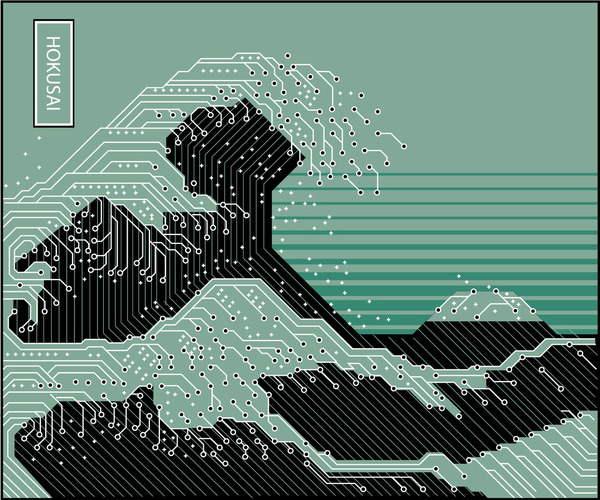
\includegraphics[width=0.82\hsize]{fig/hokusai}
\caption{"Katsushika Hokusai Electronic Circuit Board" - Joel Betancourt znany jako Garabating\label{RYS.1}}
\source{\url{https://garabating.com/post/44549621917/katsushika-hokusai-electronic-circuit-board}}
\end{figure}

% ROZDZIAŁ 1

\chapter{Cel i zakres pracy magisterskiej}

Celem niniejszej pracy jest stworzenie łatwego do rozbudowania i spójnego systemu umożliwiającego import plików projektowych używanych bezpośrednio w przemyśle PCB do programu Blender, następnie interpretację i wyświetlenie pełnowymiarowego modelu 3D płytki drukowanej która powstałaby w procesie produkcji przemysłowej. Dodatek będzie posiadał prosty i przejrzysty interfejs który zapewnia dostęp do wszystkich funkcjonalności, ale nie przytłacza odbiorcy nadmiarem funkcji. Pozwoli to nie tylko osobom technicznym z poza branży grafiki komputerowej na łatwy dostęp do wizualizacji i edycji swoich projektów ale także na łatwiejszą integrację projektów przemysłowych z marketingową i graficzną częścią przemysłu.

% Opcje programu z punktu widzenia użytkownika
\section{Wymagania funkcjonalne}

Zrealizowany system jest dodatkiem (ang. \emph{add-on}) do programu Blender, kompatybilnym z wersją 2.8 wzwyż. Wybór konkretnie tej wersji programu był podyktowany jego nową odsłoną oferującą między innymi duże zmiany w interfejsie programistycznym aplikacji (ang. \emph{API}). Wtyczka udostępnia użytkownikowi dodatkowe funkcjonalności z poziomu graficznego interfejsu programu. Następujące wymagania zostały sformułowane z punktu widzenia użytkownika.
\begin{itemize}
\item Wybranie folderu zawierającego wszystkie pliki projektu PCB lub wybranie pojedynczych plików warstw i  plików pozycji elementów (ang. \emph{"Pick And Place"})\footnote{\,Więcej o strukturze plików projektowych PCB w punkcie 1.2.3}
\item Wybranie wbudowanej lub własnej biblioteki modeli 3D
% Wyjaśnić czym jest biblioketa modeli?
\item Wybór końcowej rozdzielczości i miejsca zapisu plików wytworzonych w procesie renderowania
\item Przycisk tworzący model 3D płytki na podstawie wybranych plików
\end{itemize}

\begin{figure}[!tbh]
\centering
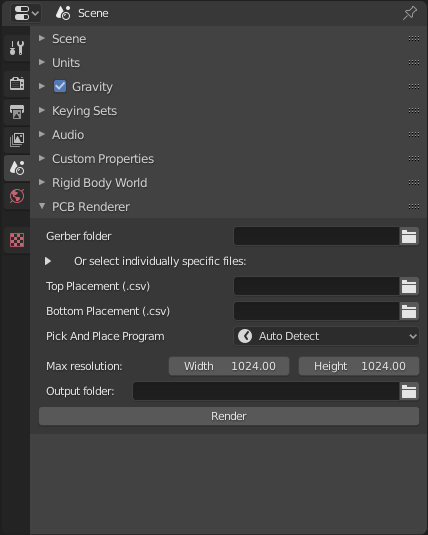
\includegraphics[width=0.75\hsize]{fig/addon_1}
\caption{Zainstalowany dodatek w programie Blender 2.82a}
\source{Opracowanie własne}
\end{figure}

\section {Opis technologii wykorzystanych w pracy}

% Python
\subsection{Python}
Python jest językiem programowania wysokiego poziomu, posiadającym aktywną społeczność i nieograniczone możliwości poprzez rozbudowę go o zewnętrzne pakiety.\footnote {\,\url{https://www.python.org/about/}} API Blendera jest w większości przygotowane do użycia właśnie Pythona i chociaż istnieją ograniczenia tego, do jakich funkcjonalności programu mamy dostęp, jest to jedyne oficjalnie wspierane rozwiązanie dzięki któremu wiele można osiągnąć bez konieczności zagłębiania się w kod C / C++ Blendera.

% Blender
\subsection {Blender 2.8}
Darmowy program \emph{Open-source}\footnote{\,\url{https://www.blender.org/about/license/}} cechujący się wszechstronnością i możliwością rozbudowania go o dodatkowe biblioteki lub skrypty napisane w języku Python, które rozszerzają podstawowe funkcjonalności.

Dodatek do programu Blender różni się od dodatkowej biblioteki Pythona jedynie pewnymi dodatkowymi wymaganiami jak obiekt zawierający metadane, takie jak: nazwa, wersja, kategoria, autor, etc. Określa też minimalną wersję Blendera wymaganą do uruchomienia skryptu. Dodatek jest więc sposobem na enkapsulację modułu Pythona w sposób, który użytkownik może z łatwością wykorzystać.

Blender ma wbudowany interpreter Pythona, który jest ładowany po uruchomieniu programu. Utrudnia to znacząco wykorzystanie automatycznego pobierania i instalowania zależnych od siebie pakietów, co za tym idzie, tworzony w ramach pracy system, aby ułatwić korzystanie z niego, musi być niezależny od zewnętrznych, dynamicznie pobieranych bibliotek.


% Gerber, G-code, CN/CNC Drill, Placement, WRL(VRML)
\subsection{Pliki projektowe PCB}

\subsubsection {Gerber}
Nowoczesne płytki drukowane są projektowane przy pomocy dedykowanego oprogramowania a ostatnim etapem produkcji dla projektanta jest wygenerowanie między innymi plików Gerber \cite{Khandpur}.
Jest to otwarty, wektorowy, powszechnie stosowany format o standardzie ASCII, służący do przesyłania danych projektowych obwodów drukowanych do przemysłu produkcji elektroniki. Wszystkie systemy do projektowania obwodów drukowanych pozwalają na eksport projektu jako pliki Gerber i każde przemysłowe oprogramowanie do ich obróbki potrafi je interpretować, umożliwiając profesjonalistom w dziedzinie PCB bezpieczną i wydajną wymianę danych projektowych \cite{Williams}.

Płytki drukowane mogą być jednostronne (jedna warstwa miedzi), dwustronne (dwie warstwy miedzi po obu stronach warstwy podłoża) lub wielowarstwowe (zewnętrzna i wewnętrzna warstwa miedzi, naprzemiennie z warstwami podłoża) \cite{schroeder}.

Pliki Gerber reprezentują między innymi warstwy miedzi, maskę lutowniczą, legendę oraz dane wiercenia i trasy. Dodatkowe atrybuty dostarczają informacji o sposobie montowania, połączeń i nazw poszczególnych elementów. Format pliku Gerber jest prosty, kompaktowy i jednoznaczny. Jest bazowany na języku \emph{G-code}, oznaczanym RS-274. Dzięki zastosowaniu 7-bitowych znaków ASCII jest czytelny dla człowieka i łatwy do debugowania. Obecnie używany od 2014 roku format to tzw. Rozszerzony Gerber (ang. \emph{Extended Gerber}) lub RS-274X.\footnote{\,Dokumentacja formatu Gerber - \url{https://www.ucamco.com/en/gerber}}

\subsubsection {Drill}
Kolejnym, generowanym przez projektanta płytki formatem używanym w produkcji są pliki wierceń (ang. \emph{NC / CNC drill}), pierwotnie zaprojektowane przez twórców wiercących i trasujących maszyn CNC jako zastrzeżone, dedykowane formaty wejściowe dla ich urządeń. Znane są pod nazwami takimi jak: Excellon, Hitachi, Sieb \& Meyer, Posalux, itd.\cite{Charras}. Wszystkie z pośród tych formatów są podobne, ponieważ opierają się na wspomnianym wcześniej G-code. Rodzaje wierceń w PCB dzielą się na otwory zwykłe - NPTH (ang. \emph{Not Plated Through Hole}) i pokryte miedzią - PTH (ang. \emph{Plated Through Hole})\cite{voldman}. Stosowanie innego standardu nie jest jednak konieczne, jako że z czasem formaty te zmieniły swoje zastosowanie i obecnie powszechnie stosowaną praktyką jest generowanie tych plików w formacie Gerber.

\subsubsection {Placement}
Ostatnim i dosyć kluczowym elementem są pliki wskazujące elementy rozmieszczane na płytce. Jest to prosty format nazywany \emph {Pick-And-Place, Placement list, X-Y file, Mount SMD}  i składa się z kilku wartości:
\begin{itemize}
\item \emph{Ref / Designator} - Indeks elementu na płytce i w projekcie
\item \emph{Value} - Wartość elementu (np. pojemność, rezystancja, napięcie)
\item Pozycja podana we współrzędnych kartezjańskich
\item \emph{Footprint / Package} - Nazwa elementu, zazwyczaj zawiera także informację o jego wymiarach
\item Rotacja elementu
\item Informacja czy objekt znajduje się na wierzchniej czy też dolnej stronie płytki
\item Ewentualne komentarze i dodatkowe informacje
\end{itemize}
Plik zawiera opis elementów montowanych za pomocą technologii montażu przewlekanego - THT (ang. \emph{Through-hole technology}) oraz powierzchniowego - SMT (ang. \emph{Surface Mount Technology}), powszechnie stosowanego przemysłowo \cite {prasad}. Nie jest to jednak format ściśle ustandaryzowany i przy masowej produkcji każdy producent musi manualnie zweryfikować opisy elementów. Na szczęście każdy program do tworzenia PCB posiada eksporter do generowania tychże plików. Dodatkowo są one proste w zapisie i z łatwością edytowalne przez człowieka.

\subsection{Pliki VRML i X3D}
Format \emph{.wrl} zwany VRML (ang. \emph {Virtual Reality Modeling Language}) powstały w 1994 roku, stał się pierwszym internetowym formatem 3D, został później zastąpiony przez format X3D \cite{vrml}. Jego ówczesna powszechność sprawiła, że wiele programów przemysłowych tworzonych w latach dziewięćdziesiątych posiada bazy modeli w tym właśnie formacie. Więcej o praktycznym wykorzystaniu tego standardu w rozdziale \ref{wrl}.

\subsection{Środowisko Visual Studio Code}
Visual Studio Code jest to darmowy edytor kodu który według badań przeprowadzanych co roku przez serwis StackOverflow\footnote{\,\url{https://insights.stackoverflow.com/survey/2018/\#development-environments-and-tools}}$^{,}$\footnote{\,\url{https://insights.stackoverflow.com/survey/2019\#development-environments-and-tools}} cieszy się coraz większym uznaniem. Wybór tego środowiska nie był jednak dyktowany jego popularnością lecz nowymi możliwościami otwierającymi się dzięki instalowaniu w nim rozszerzeń.\footnote{\,\url{https://code.visualstudio.com/docs/editor/extension-gallery}} Dodatek stworzony przez Jacques Lucke na potrzeby rozwoju addonów do programu Blender pozwala między innymi na automatyzację procesu aktualizowania tworzonego addonu przez tworzenie skrótu w wewnętrznych folderach Blendera, co znacznie przyśpiesza pracę nad systemem. Ponadto posiada ułatwienia takie jak debugowanie w konsoli, tworzenie odpowiednich struktur i przydatne komendy. Sposób działania dodatku ma na celu także upewnienie się, że rozszerzenie nie koliduje z innym menedżerem pakietów Pythona.\footnote{\,\url{https://marketplace.visualstudio.com/items?itemName=JacquesLucke.blender-development}} 

\chapter{Architektura zrealizowanego systemu}
Aby zobrazować podstawowe założenia projektu, w niniejszym rozdziale zostanie omówiona koncepcyjna struktura zrealizowanego systemu. Przedstawi ona bardziej szczegółowo mechanizmy działania najważniejszych komponentów aplikacji, a finalnie pomoże w samym procesie tworzenia oprogramowania.

\section{Założenia i wymagania projektowe}
W przypadku tak rozległych możliwości rozwoju systemu, kluczowe jest właściwe zdefiniowanie wymagań projektu i dążenie do ich realizacji. Postawienie ograniczeń w kwestii wspieranych formatów na jakich działał będzie dodatek jest konieczne z uwagi na zróżnicowanie technologii używanych w procesie tworzenia PCB. Z drugiej strony nacisk na modułowość rozwiązania pozwoli później na łatwiejsze dodanie dowolnego rozszerzenia.
System powinien implementować wszystkie następujące funkcjonalności:

\begin{itemize}

\item Implementacja interfejsu przy pomocy API Blendera 2.8

\item Czytanie i interpretacja plików Gerber (RS-274X)

\item Tworzenie modelu płytki na podstawie otrzymanych plików, zgodnego z rzeczywistymi wymiarami

\item Czytanie i interpretacja pliku placement w formacie \emph{.csv}

\item Udostępnienie użytkownikowi możliwości użycia dostarczonej lub własnej bazy modeli podzespołów

\end{itemize}

\section {Struktura projektu}
Podstawowy wybór strukturalny następującego rozwiązania jest podyktowany wymaganiami i sposobem komunikacji z API Blendera. Struktura folderów dodatku do programu Blender jest dowolna z założeniem, że w folderze głównym znajduje się plik \emph{\_\_init\_\_.py} odpowiedzialny za rejestrowanie dodatku. Jest on automatycznie wykonywany po wybraniu folderu i włączeniu addonu w sekcji "Dodatki" w programie Blender. Pozostałe elementy są pogrupowane według konwencji modułów w języku Python, zatem każdy moduł posiada swój folder, jest to jednak podyktowane tylko enkapsulacją modułów i wygodą w używaniu referencji między skryptami.

\subsection{Główna struktura interfejsu API Blendera}
Z poziomu kodu, API Blendera udostępnia główne moduły pod słowem kluczowym \textbf{bpy}\footnote{\,\url{https://docs.blender.org/api/current/index.html}} a jego podstawowe i główne elementy to:
\begin{itemize}
\item \textbf{bpy.data} -- Zapewnia dostęp do danych bieżącego pliku \emph{.blend} (Jest to rozszerzenie używane przez program Blender). Każde z jego pól jest zbiorem obiektów danego typu (sceny, obiekty, zbiory wierzchołków, materiały, kolekcje itp.).
\item \textbf{bpy.context} -- Zawiera wszelkie dane środowiskowe obrazujące bieżący stan programu (bieżący wybór, tryb i region edytora) oraz wiele globalnych właściwości takich jak: preferencje użytkownika, bieżące ustawienia sceny.
\item \textbf{bpy.ops} -- Zawiera wszystkie \emph{Operatory} Blendera. (W API każda komenda Blendera jest zaimplementowana jako metoda klasy \emph{Operator}).
\item \textbf{bpy.types} -- Posiada definicje wszystkich klas używanych w strukturach.
\end{itemize}
Istnieje także wiele mniejszych, pobocznych modułów i podmodułów pomocniczych. Niektóre z nich nie należą nawet do głównego modułu \textbf{bpy}. Mniejsze moduły, między innymi: bpy.props, bpy\_extras, bpy.utils, mathutils, bmesh, będą omówione w dalszej części tej pracy.

API Blendera wymaga od klas implementacji ściśle zdefiniowanych metod. Jest to rodzaj „umowy” pomiędzy skryptem a systemem rdzenia Blendera. Zgadzamy się na wdrożenie wymaganych funkcji w swojej klasie a Blender zgadza się wywoływać je w ściśle określonych okolicznościach. W programowaniu obiektowym taka lista zakontraktowanych funkcji i właściwości nazywa się „interfejsem”. Aby pomóc w jego implementacji, API Blendera dostarcza odpowiednie klasy bazowe, które w żargonie programowania obiektowego są tak zwanymi „klasami abstrakcyjnymi”. Zapewniają domyślne, puste implementacje wszystkich metod wymaganych przez interfejs. Nasze klasy dziedziczą tę domyślną treść z klasy bazowej.

\subsection{Implementacja wzorca projektowego} \label{mvp}
MVP (ang. \emph{Model–view–presenter}) jest wzorcem architektury oprogramowania opierającym się na trzech głównych założeniach\cite{mvp}:
\begin{itemize}
\item Model reprezentuje dane które są przetwarzane i wysyłane do prezentera
\item Widok (\emph{View}) wyświetla dane uzyskane z prezentera i przekazuje dane wejściowe wprowadzane przez użytkownika do prezentera
\item Prezenter jest wywoływany z Widoku aby wyświetlać dane pobrane z Modelu i przetwarzać dane wejściowe
\end{itemize}
System został zaimplementowany w oparciu o ten właśnie wzorzec z uwagi na to, że jest to struktura logicznie wynikająca ze sposobu używania API Blendera.
W tym przypadku, w dużym uproszczeniu Modelem jest logika modułu, Widokiem -- klasa odpowiedzialna za renderowanie i odbieranie danych wejściowych a Prezenter to API Blendera.
\newline


Skrypty w języku Python można zintegrować z Blenderem na następujące sposoby:
\begin{itemize}
\item Definiując silnik renderujący
\item Poprzez zdefiniowanie operatorów
\item Poprzez zdefiniowanie menu, nagłówków i paneli
\item Wstawiając nowe przyciski do istniejących menu, nagłówków i paneli
\end{itemize}

Odbywa się to poprzez zdefiniowanie klasy, która jest podklasą istniejącego typu.
Tak więc, przechodząc do rzeczywistego stanu rzeczy, omawiany addon o nazwie \emph{PCB-Blender} jest zdefiniowany jako skompresowane archiwum składające się z następujących elementów:
\begin{itemize}
\item \emph{PCB\_LayoutPanel} -- Klasa odpowiedzialna za wyświetlanie interfejsu i przekazywanie danych wybranych przez użytkownika, dziedzicząca z klas abstrakcyjnych \emph{Panel} i \emph{ImportHelper}. Wraz z klasami pomocniczymi znajduje się w pliku PCB\_Blender\_panel.py.
\item \emph{PCB\_Generate} -- Klasa dziedzicząca z klasy \emph{Operator}, znajdująca się razem z klasami pośrednimi w pliku PCB\_Blender.py.
\item \emph{\_\_init\_\_.py} -- Plik zawierający metadane i rejestrujący powyższe klasy,
\item Foldery zawierające pozostałe moduły Pythona do których odnosi się główny Operator -- \emph{PCB\_Generate}.
\end{itemize}

\subsection{Baza modeli}

Jednym z pierwszych z wyzwań podczas tworzenia dodatku był dobór zasobów w postaci modeli 3D. Aby zrealizować założenia pracy, wymagana była baza modeli podzespołów elektronicznych montowanych na PCB. Z uwagi na mnogość producentów, rodzajów i typów podzespołów oraz fakt, że każdy program służący do projektowania może oznaczać je inaczej, optymalnym rozwiązaniem wydaje się udostępnienie użytkownikowi podstawowej bazy modeli. Ponadto zastosowanie szukania modeli częściowo dopasowanych nazwą. Z uwagi na fakt, że niemożliwym jest obsługa wszystkich wyjątków, koniecznością staje się umożliwienie użytkownikowi kożystanie z własnych, wybranych modeli. Istnieje wiele stron udostępniających modele 3D na zasadach komercyjnych jak i darmowych licencji. Są one często wykorzystywane przez twórców jak i programy projektowe. Oto kilka z nich zaprezentowanych w tabeli: \ref{fig:table}.

\begin{table}[htb]
\begin{tabular}{|l|l|l|} \hline
Adres URL \\ \hline
\url{https://grabcad.com/} \\ \hline
\url{https://www.3dcontentcentral.com/} \\ \hline
\url{https://www.digikey.com/en/resources/3d-models} \\ \hline
\url{https://www.te.com/} \\ \hline
\url{https://www.traceparts.com/en} \\ \hline
\end{tabular}
\caption{Publicznie dostępne bazy modeli podzespołów}
\source{Opracowanie własne}
\label{fig:table}
\end{table}
Nie posiadają one jednak możliwości masowego pobierania modeli. Pomijając tą niedogodność, która musiałaby być rozwiązana skryptem automatyzującym pracę, również ilość pobranych materiałów znacznie przekroczyłaby racjonalny poziom. Z pomocą przychodzi tu darmowy zbiór modeli używanych w programie KiCad\footnote{\,\url{https://kicad.github.io/packages3d/}}. Modele są dostępne między innymi w formacie \emph{.wrl} więc można zaimportować je do Blendera. Więcej o przetwarzaniu plików \emph{.wrl} oraz tworzeniu bazy modeli w rozdziale \ref{wrl}.



\chapter{Szczegóły implementacyjne systemu}
W tym rozdziale zostanie omówiona implementacja kluczowych i pobocznych funkcjonalności systemu. Sposób implementacji narzucony przez wybrany wzorzec projektowy wpasowuje się w przyjęte i zalecane praktyki programowania obiektowego jak również tworzenia dodatków w Blenderze. Dzięki przyjętym wcześniej założeniom, funkcjonalności programu zostały podzielone na niezależne części których implementacja zostanie teraz przedstawiona. Niniejszy rozdział zastał podzielony na fragmenty przedstawiające: rejestrowanie dodatku, implementację interfejsu, renderowanie PCB, tworzenie bazy modeli oraz rozważania na temat dalszych możliwości rozwoju stworzonego rozwiązania.


\section {Rejestrowanie addonu}
Zgodnie z dokumentacją, każdy dodatek do Blendera musi posiadać obiekt \emph{bl\_info}, zawierający metadane addonu i implementować metody \emph{register} oraz \emph{unregister}. Instalacja dodatku następuje poprzez wybranie folderu dodatku, wówczas dodatek zostaje dodany do listy wyświetlającej między innymi metadane dostarczone w obiekcie \emph{bl\_info}. Po aktywowaniu dodatku w programie zostaje wykonana metoda \emph{register} i analogicznie \emph{unregister} w przypadku usuwania addonu. Wprowadzone w wersji 2.8 API Blendera usprawnienia znacznie ułatwiają ten proces. Jeżeli nie są wymagane dodatkowe funkcjonalności podczas rejestrowania i usuwania dodatku lub jego komponentów, istnieje możliwość użycia funkcji \emph{register\_classes\_factory} z pakietu \textbf{bpy.utils}, która automatycznie je zaimplementuje. Poniżej przedstawiony jest w całości plik odpowiedzialny za instalowanie, włączanie i wyłączanie dodatku.

\lstset{caption={\emph{\_\_init\_\_.py} -- Plik rejestrujący dodatek.}}
\begin{lstlisting}
bl_info = {
	"name" : "PCB-Blender",
	"author" : "Adam Makiewicz",
	"description" : "Addon for generating models of PCB from Gerber files",
	"blender" : (2, 80, 0),
	"version" : (0, 1, 4),
	"category" : "Generic",
	"location" : "Scene Properties > PCB Renderer"
}
	import bpy
	from . PCB_Blender_panel import PCB_LayoutPanel
	from . PCB_Blender import PCB_Generate

	classes = (PCB_LayoutPanel, PCB_Generate)
	register, unregister = bpy.utils.register_classes_factory(classes)
\end{lstlisting}
\source{Opracowanie własne}
\section {Implementacja interfejsu}

Klasa \emph{PCB\_LayoutPanel} dostarcza całą funkcjonalność renderowania interfejsu dzięki dziedziczeniu z wewnętrznej klasy bazowej \emph{Panel}. Poprzez implementację tej klasy, w programie zostaje utworzony panel w wybranym regionie. Właściwości takie jak nazwa, miejsce wyświetlania się panelu, wielkość, kontekst, typ regionu itp. muszą być zdefiniowane w odpowiednim formacie. Dzięki temu są one automatycznie interpretowane przez API i poprawnie wyświetlane. Właściwości klasy zaczynają się od przedrostka \emph{bl\_}, jest to konwencja używana w celu odróżnienia wbudowanych właściwości wewnętrznych klas Blendera od tych, które zostają dodane przez programistę. Przykład implementacji wbudowanych właściwości klasy dziedziczącej znajduje się poniżej.
\newpage
\lstset{caption={Właściwości panelu z pliku \emph{PCB\_Blender\_panel.py}}}
\begin{lstlisting}
class PCB_LayoutPanel(Panel):
	bl_label = "PCB Renderer"
	bl_idname = "SCENE_PT_layout"
	bl_space_type = 'PROPERTIES'
	bl_region_type = 'WINDOW'
	bl_context = "scene"
\end{lstlisting}
\source{Opracowanie własne}
\vspace{5mm}

Oprócz posiadania statycznych właściwości, klasa powinna przechowywać i przekazywać dynamiczne zmienne. Aby dodać zmienną do zarejestrowanej klasy w Blenderze należy użyć jednej z Definicji Właściwości (ang. \emph{Property Definition}) z modułu \textbf{bpy.props}. Moduł ten definiuje właściwości rozszerzające wewnętrzne dane Blendera. Wynik tych funkcji służy do przypisywania właściwości do klas zarejestrowanych w Blenderze i nie można ich używać bezpośrednio. Są to między innymi \emph{StringProperty, FloatProperty, EnumProperty, BoolProperty} lub dowolne ich zestawienie jako jedna strukturalna zmienna. Funkcje wymagają każdorazowego zdefiniowania nazwy, opisu, wartości domyślnej, podtypu itp. więc aby uniknąć redundancji kodu zostały stworzone funkcje pomocnicze, przedstawione we fragmencie kodu \ref{Listing3}. Zdefiniowanie typu \emph{StringProperty} jako ścieżka do pliku lub folderu sprawia, że do elementu wyświetlającego tą zmienną automatycznie zostanie przypisany przycisk otwierający eksplorator plików w celu wybrania pliku.

\lstset{caption={Funkcje pomocnicze tworzące zmienną o tym samym typie lecz innym zastosowaniu -- ścieżka pliku i ścieżka folderu}\label{Listing3}}
\begin{lstlisting}
def FilePath(_name, _description="", _default=""):
	return StringProperty(name=_name, default = _default,
	description=_description, subtype = 'FILE_PATH')
    
def DirPath(_name, _description="", _default=""):
	return StringProperty(name=_name, default = _default,
	description=_description, subtype = 'DIR_PATH')
\end{lstlisting}
\source{Opracowanie własne}

Oprócz zmiennych, aby poprawnie zaimplementować dany interfejs, klasa musi zawierać też funkcję \emph{draw} odpowiedzialną za renderowanie elementów w panelu. Wygląd i rozmieszczenie obiektów jest zdefioniowany przy pomocy obiektu klasy \emph{UILayout} i jego elementów takich jak kolumny i rzędy w których umieszcza się referencje do wspomnianych wyżej, dynamicznych zmiennych. 
W elementach układu można umieszczać opisy, ikony a nawet definiować ich zachowanie przy pomocy instrukcji warunkowych. Poniżej znajduje się fragment kodu, używający zmiennej \emph{boolowskiej} oraz instrukcji warunkowej w celu zdefiniowania zachowania listy rozwijanej.

\lstset{caption={Fragment kodu z klasy \emph{PCB\_LayoutPanel} definiujący zachowanie się rozwijalnej listy elementów}\label{Listing4}}
\begin{lstlisting}
row = layout.row()
	row.prop(context.scene, "expand", icon="TRIA_DOWN"
	if context.scene.expand
	else "TRIA_RIGHT", icon_only=True, emboss=False)
	row.label(text="Or select individually specific files:")

	if bpy.context.scene.expand:
		col = layout.column()
		col.label(
		text="To use gerber folder, collapse this section!",
		icon='ERROR')
\end{lstlisting}
\source{Opracowanie własne}

Następnie w jednym z elementów zostaje umieszczone wywołanie operatora z klasy \emph{PCB\_Generate}, który przyjmuje kontekst w którym zostal wywołany --- a zatem również wszystkie zmienne.

% mogę to bardziej rozpisać i dać przykłady, ale są to bardzo proste i trywialne jednolinijkowce. 

\section {Tworzenie PCB}
Jak wspomniano wcześniej, funkcja wykonania operatora (\emph{execute}) pobiera w argumencie informacje o środowisku i bieżący kontekst w jakim jest wywoływana. Następnie wykonuje w programie odpowiednie obliczenia i przekształcenia, które zostały podzielone na następujące kategorie:
\subsection{Funkcje użytkowe}
Tak samo jak w przypadku klasy odpowiedzialnej za renderowanie interfejsu, tutaj też zostały stworzone funkcje pomocnicze w celu uniknięcia powtarzalności kodu oraz zwiększenia czytelności przebiegu całego programu. Są one używane w obrębie całego projektu.
\subsubsection{Funkcje informacyjne}
Wszystkie z tych funkcji odnoszą się do obiektu klasy \textbf{bpy.context.window\_manager}.
\begin{itemize}
\item Funkcje \emph{RegisterProgress, UpdateProgress} oraz \emph{EndProgress} służą do wyświetlania kursora postępu podczas wykonywania obliczeń i są używanie na przestrzeni wszystkich innych funkcji o znaczącej złożoności.
\item Funkcja \emph{ShowMessageBox} jest używana we wstępnej fazie walidacji otrzymanych zmiennych zanim zostaną wywołane pozostałe funkcje obliczające. Służy do wyświetlenia komunikatu informacyjnego lub błędu. Zazwyczaj zestawiona z anulowaniem lub przerwaniem wykonywania obliczeń, objaśniająca użytkownikowi powód zaprzestania działania.
\end{itemize}
\subsubsection{Funkcje edytujące}
Funkcje odnoszące się do bieżącego kontekstu i modyfikujące go wraz ze stanem aplikacji.
\begin{itemize}
\item \emph{DeselectAll} --- Odznacza wszelkie obiekty aktywne na scenie, przydatna funkcjonalność gwarantująca powtarzalność wykonywanych operacji bez znaczenia w jakim stanie początkowym użytkownik uruchomi polecenia generujące obiekty.
\item \emph{ChangeArea} --- Zmienia tryb okna wyszukując obecny aktywny region w kontekście.
\item \emph{ChangeClipping} --- Modyfikuje minimalną odległość od renderowanego obiektu w oknie widoku do jakiej może zbliżyć się kamera. Podstawową wartością w Blenderze jest 10 centymetrów co jest zazwyczaj zbyt dużą odległością na oglądanie płytki drukowanej rzeczywistych wymiarów.
\item \emph{PurgeOrphanData} --- Funkcja czyszcząca pamięć podręczną programu z nieużywanych na scenie elementów (wytworzonych obiektów, siatek modeli, zaimportowanych zdjęć i dołączonych plików \emph{.blend}). Nie jest ona obecnie wywoływana podczas przebiegu programu, jednak jest używana w procesie rozwoju i testowania aplikacji, ułatwiając resetowanie stanu całego programu w celu uzyskania powtarzalności testów.
\end{itemize}
\subsection{Interpretacja plików}
\subsubsection{Placement}

O ile pliki placement i ścieżka do bazy modeli 3D zostały zapewnione, program uruchomi metodę \emph{ReadPlacement\_csv}, przeczyta plik \emph{.csv}, zarejestruje nazwy, numery porządkowe, pozycje i rotacje wymaganych komponentów. Nazwy plików muszą zostać przycięte do dlugości 63 znaków, ponieważ jest to limit długości nazwy obiektu w wewnętrznej strukturze Blendera. Następnie, przeszukując rekursywnie folder wskazany jako baza modeli, dołączy wszystkie znalezione pliki \emph{.blend}, jednocześnie sprawdzając czy plik posiada szukany obiekt. Nie są to operacje rzutujące na ilość alokowanej pamięci ponieważ tworzą tylko połączenia z plikiem źródłowym, jednak wraz ze wzrostem ilości przeszukiwanych plików, znacząco wzrasta czas wykonywanych operacji.

W przypadku gdy któryś z modeli nie został znaleziony jest uruchamiana funkcja wyszukiwania modelu o podobnej nazwie. Jest to algorytm, który porównuje początek nazwy obiektu, jednak dzięki uwzględnieniu stosowanej konwencji w nazewnictwie modeli podzespołów, jest w stanie osiągnąć o wiele mniejszą złożoność czasową niż podstawowy algorytm naiwny. Nazwy komponentów są to zazwyczaj ciągi nazw i oznaczeń oddzielone znakami "\_".

\lstset{caption={Algorytm wyszukiwania komponentu po nazwie z uwzględnieniem całych słów oddzielanych separatorem "\_"}}
\begin{lstlisting}
for missing in required:
    separatedList = missing.split('_')
    for compfile in compfiles:
        UpdateProgress(i/len(compfiles))
        found = False
        with bpy.data.libraries.load(compfile, link=True)
        as (data_from, data_to):
            i = 0
            # Search models with names starting with most keywords possible
            while i < len(separatedList)-1:
                newSearch = separator.join
                (separatedList[:len(separatedList)-i])
                newFound = [value for value in
                data_from.meshes if value.startswith(newSearch)]
                if len(newFound) > 0:
                    elementFound = min(newFound, key=len)
                    requested  = separator.join(separatedList)
                    print("Found: ", elementFound,
                    " similar to requested: ", requested)
                    data_to.meshes.append(elementFound)
                    for col in layout_table:
                        if col[2] == requested:
                            col[2] = elementFound
                    found = True
                    break
                else:
                    i+=1
        if found:
            break
\end{lstlisting}
Po uzyskaniu listy modeli, program ustawia je w odpowiednich miejscach zgodnych z wcześniej przeczytanymi koordynatami, uwzględniając ich rotację oraz skalę. Skala komponentów różni się w zależności od tego jaki typ jednostki jest używany w projekcie (milimetr lub mil --- 1/1000 cala). W przypadku braku modelu, w odpowiednie miejsce zostaje ustawiony pusty obiekt, posiadający nazwę i numer porządkowy.
Wczytane modele oraz informacje o dołączonych plikach \emph{.blend} są zapisywane w tak zwanej pamięci podręcznej (ang. \emph{cache}) programu. Sprawia to, że kolejna operacja wczytująca modele nie musi dodawać więcej plików z bazy modeli oraz ładować siatki już użytych modeli komponentów. Dzięki temu kolejne użycie programu (bez wyłączania go) jest znacznie szybsze.
% TODO: Opisać to szczegółowo? kod?
\subsubsection{Gerber}
Do wczytania plików Gerber i Excellon został wykorzystany moduł Pythona \emph{pcb-tools 0.1.6}, stworzony przez Paulo Henrique Silva i udostępniony na zasadach licencji Apache\footnote{\,\url{https://pypi.org/project/pcb-tools/}}. Narzędzia udostępniane przez moduł pozwalają na interpretację instrukcji G-code zawartych w plikach i zamianę ich na obiekty. Moduł, aby umożliwić mu funkcjonowanie w ramach projektu, został zmodyfikowany. Modyfikacje obejmują:
\begin{itemize}
\item Statyczne dołączenie bibliotek używanych przez moduł
\item Zmiany nagłówków sktyptów, aby wskazywały na dołączone moduły
\item Dodanie słów kluczowych do słownika wyszukującego i klasyfikującego typy warstw po nazwie pliku, w skrypcie \emph{layers.py}
\item Lustrzane odbicie dolnej warstwy renderowaniej płytki\footnote{Dolne warstwy płytek w programach projektujących są tworzone w odbiciu lustrzanym aby wprowadzić przejrzystość. Projektowanie odbywa się zazwyczaj w widoku rzutu z góry.}
\item Przechwytywanie danych wyjściowych w celu zapisu do pliku w formacie \emph{.PNG}
\item Dodana obsługa wykrywania obramowania płytki na podstawie wczytanych warstw, na wypadek gdyby warstwa odpowiedzialna za kształt nie została znaleziona (przedstawiona we fragmencie kodu \ref{Listing5})
\end{itemize} 

\lstset{caption={Obliczanie obramowania płytki na podstawie warstw}\label{Listing5}}
\begin{lstlisting}
x_range = [10000, -10000]
y_range = [10000, -10000]
for layer in layers:
	bounds = layer.bounds
	if(self.first_bounds is None):
		self.first_bounds = bounds

	if self.first_bounds is not None:
		layer_x, layer_y = self.first_bounds
		x_range[0] = min(x_range[0], layer_x[0])
		x_range[1] = max(x_range[1], layer_x[1])
		y_range[0] = min(y_range[0], layer_y[0])
		y_range[1] = max(y_range[1], layer_y[1])
width = x_range[1] - x_range[0]
height = y_range[1] - y_range[0]

scale = math.floor(min(float(max_width)/width, float(max_height)/height))
self.scale = (scale, scale)
\end{lstlisting}

W procesie interpretacji pliku zostaje utworzona nowa instancja klasy \emph{PCB}, która będzie zawierała między innymi obiekty reprezentujące poszczególne warstwy i funkcje wskazujące odpowiednie grupy warstw. Typy warstw są rozpoznawane przez program przy pomocy wyszukiwania wzorca w jego nazwie. W przyszłości możliwe jest dodanie wyszukiwania wzorca także w treści pliku. Byłaby to niezawodna i uniwersalna, lecz skomplikowana i czasochłonna operacja. Wszystkie fragmenty tekstu są porównywane za pomocą wyrażeń regularnych zdefiniowanych w słowniku, znajdującym się w pliku \emph{layers.py}. Fragment kodu \ref{Listing6} pokazuje główną funkcję, odpowiedzialną za definiowanie typu warstwy.

Każdej warstwie zostaje przydzielony typ (określający sposób w jaki będzie musiała zostać później wyrenderowana) oraz grupa obiektów 2D opisujących kształty --- tzw. prymitywy (ang. \emph{primitives}), składające się z wielokątów i krzywych o różnych grubościach. Ostatecznie warstwy są sortowane w odpowiedniej kolejności i dzielone na grupy: górne, dolne, wiercenia, i kontur.

\newpage
\lstset{caption={Funkcja klasyfikująca warstwę do odpowiedniej kategorii.}\label{Listing6}}
\begin{lstlisting}
def guess_layer_class(filename):
    try:
        layer = guess_layer_class_by_content(filename)
        if layer:
            return layer
    except:
        pass
    try:
        directory, filename = os.path.split(filename)
        name, ext = os.path.splitext(filename.lower())
        for hint in hints:
            if hint.regex:
                if re.findall(hint.regex, filename, re.IGNORECASE):
                    return hint.layer
            patterns = [r'^(\w*[.-])*{}([.-]\w*)?$'
                       .format(x) for x in hint.name]
            if ext[1:] in hint.ext 
            or any(re.findall(p, name, re.IGNORECASE) for p in patterns):
                return hint.layer
    except:
        pass
    return 'unknown'
\end{lstlisting}

\subsubsection{Renderowanie}
\emph{Cairocffi} jest to oparty o CFFI\footnote{\,Interfejs do języka Python, umożliwiający wywoływanie metod w języku C}$^{,}$\footnote{\,\url{https://cffi.readthedocs.io/en/latest/}} zamiennik modułu \emph{Pycairo} --- zestawu powiązań Pythona i obiektowego API dla \emph{Cairo}. \emph{Cairo} jest to biblioteka grafiki wektorowej 2D z obsługą wielu formatów wyjściowych, w tym buforów obrazów, plików \emph{PNG, PostScript, PDF} i \emph{SVG}. 
Klasa \emph{GerberCairoContext} w pliku cairo\_backend.py odpowiada za powiązania funkcji renderowania obiektów bezpośrednio do biblioteki \emph{Cairocffi}. Jak wspomniano wcześniej, moduł ten został statycznie dołączony do projektu.

%TODO: moar
Jeżeli użytkownik wskazał pliki warstw i wierceń lub folder je zawierający, program po wykonaniu analizy stworzy instancję obiektu PCB. Następnie jest uruchamiana metoda \emph{CreateImage} która przekazuje obiekt PCB do klasy \emph{GerberCairoContext}. Wszystkie składowe obiekty płytki

zostaną one pogrupowane w celu stworzenia dwóch obrazów płytki --- górnej i dolnej warstwy
warstwy odpowiednie właściwości i prymitywy
Każda ze składowych warstwy



Każda z warstw, wraz z należącymi do niej obiektami jest renderowana jako osobny obraz oraz nakładana na pozostałe w odpowiedniej kolejności. Efektem wyjściowym jest stworzenie dwóch obrazów w formacie \emph{.PNG}.

Pliki posiadają wcześniej zdefiniowaną rozdzielczość, a zapisane są w folderze wskazanym przez użytkownika. Nazwy plików posiadają prefiks "Top\_layer" lub "Bottom\_layer" oraz datę i czas stworzenia jako sufiks. 

Kolejnym krokiem jest stworzenie modelu płytki poprzez uruchomienie metody \emph{CreateModel}. W zależności od tego czy podczas interpretacji pliku gerber, została wykryta warstwa konturowa lub nie, zostaje stworzona siatka będąca obramowaniem płytki. W przypadku braku warstwy konturowej, wymiary siatki zostają wybrane jako punkty graniczne (ang. \emph{bounds}) obiektu PCB, to znaczy prostokątu obliczonego na podstawie maksymalnych i minimalnych koordynatów użytych we wszystkich warstwach. Model jest odpowiednio skalowany aby zachować rzeczywiste wymiary.
% ew. opisać bardziej sposób renderowania (trochę nudne) + fragment kodu?
Dwuwymiarowy kształt płytki zostaje następnie pogrubiony metodą \emph{Extrude} około 1.6 milimetra --- jest to standardowa przyjęta grubość płytki po złożeniu wszystkich warstw \cite{Khandpur}.
Ostatecznie zostają stworzone i nadane obu stronom płytki dwa materiały używające wcześniej stworzonych plików \emph{.PNG} jako tekstur. Dodatkowo jest stworzony lub załadowany (jeżeli już istnieje w pamięci podręcznej) materiał boczny imitujący kolor krzemowej płytki i przypisane są mu odpowiednie wartości.

% TODO: więcej info
\section {Baza modeli\label{wrl}}

Aby stworzyć modele komponentów i zapisać je w postaci pliku \emph{.blend} wymagane było użycie samego programu Blender. Niestety importer plików \emph{.wrl} nie działa prawidłowo (nie wczytuje materiałów, ucina modele, tworzy bardzo dużą ilość niezoptymalizowanej geometrii). Ponadto nie posiada możliwości importu wielu plików na raz.

Z uwagi na powyższe, w ramach pracy powstała zmodyfikowana wersja wbudowanego w Blendera importera plików \emph{.wrl} w celu stworzenia bazy modeli. Było to możliwe dzięki udostępnionemu publicznie kodowi Blendera. Niektóre z usprawnień zostały zaproponowane jako oficjalna zmiana w przyszłych wersjach programu Blender. Modyfikacje obejmują:
\begin{itemize}
\item Dodanie obsługi materiałów
\item Optymalizacja procesu tworzenia geometrii (usuwanie wielokrotnych wierzchołków)
\item Obsługa importu wielu plików z wybranego folderu
\item Czyszczenie pamięci (ang. \emph{garbage collection})
\item Zapisywanie materiałów tworzonych przy imporcie w pamięci podręcznej
\item Obsługa wyjątków przy wczytywaniu nietypowych lub wielokrotnie zagnieżdżonych struktur w plikach
\item Poprawne wczytywanie nazwy obiektu
\end{itemize}
% Oczywiście mogę tu rozpisać więcej informacji o tych fragmentach

\section{Możliwości dalszego rozwoju systemu}
\subsubsection{PCB-Blender}
Potencjalne dodatkowe funkcjonalności które mogą być z wprowadzone do projektu w celu polepszenia doświadczeń użytkownika i zwiększenia możliwości programu:
\begin{itemize}
\item Stworzenie kolejnych baz modeli na podstawie komponentów z innych programów projektowych.
\item Stworzenie słownika nazw modeli aby wiele nazw wskazywało na jeden model.
\item Renderowanie dowolnej ilości warstw (możliwość wybrania dowolnie wielu plików i kolejności ich renderowania).
\item Dopisywanie wyrażeń regularnych (wykrywanie i poprawna klasyfikacja większej ilości rozszerzeń i nazw plików).
\item Definiowane innych palet i schematów kolorystycznych dla renderowanych obrazów płytek.
\item Wsparcie dla innych formatów plików projektowych (moduł pcb-tools zapowiada w swoim opisie planowane wsparcie dla formatów IPC-2581, ODB++ i innych\footnote{https://pcb-tools.readthedocs.io/en/latest/about.html}).
\end{itemize}

\subsubsection{Importer formatu \emph{.WRL}}
\begin{itemize}
\item Optymalizacja --- zmniejszenie zapotrzebowanie na pamięć przy przetwarzaniu dużych plików.
\item Zmniejszenie rozmiaru plików przy pomocy instancionowaniu geometrii (wiele elementów posiada powtarzające się elementy).
\end{itemize}



% Czy dodanie gdzieś rozdziału "przegląd krytyczny literatury - analiza krytyczna dotychczasowych badań/rozwiązań z zakresu tematu" ma sens? Jeżeli tak to gdzie go wcisnąć? Znalazłem 2 addony jeżeli chodzi o kompatybilność z blenderem:  (https://bitbucket.org/hyOzd/pcb2blender/src/master/, https://github.com/majenkotech/PCB-Blend). Jest ich o wiele więcej jeżeli patrzeć by tylko na Pythona. Oba bardzo specyficzne: do gEDA i Eagle, nieposiadające interfejsu, niewygodne do użycia, wymagają dotatkowych narzędzi, znikoma dokumentacja, jednak wziąłem pomysł z jednego z nich do wczytywania modeli.

% https://bitbucket.org/hyOzd/pcb2blender/src/master/
% https://github.com/majenkotech/PCB-Blend

% pakiet modeli z gEDA https://github.com/majenkotech/PCB-Blend
% pakiet modeli z KiCAD (wrl) https://kicad.github.io/packages3d/


\summary

Praca ta omawia proces tworzenia dodatku do programu Blender. Na podstawie plików projektowych, dodatek tworzy realistyczną i wierną rzeczywistym wymiarom wizualizację modelu 3D płytki drukowanej, która powstałaby w procesie produkcji przemysłowej. W pierwszym rozdziale zostały opisane wszystkie technologie użyte podczas tworzenia oprogramowania. Dalej, została omówiona architektura realizowanego systemu, implementacja interfejsu i logiki, a także proces tworzenia zasobów w postaci bazy modeli 3D.
Aby dodatek był łatwy w użytkowaniu, całość stworzonego i opisanego w tej pracy oprogramowania, wraz z bazami modeli koniecznymi do prawidłowego wczytywania plików \emph{placement}, jest dostępna pod adresem dołączonym do pracy w załączniku \ref{linki}. 

Podsumowując, w efekcie końcowym zostały utworzone \emph{de facto} 2 dodatki. Jeden oferujący zakładaną funkcjonalność oraz drugi, powstały jako narzędzie do tworzenia bazy modeli. W wyniku prac implementacyjnych udało się zrealizować projekt, który jest zgodny z przyjętymi wcześniej wymaganiami i założeniami przedstawionymi na etapie opracowywania koncepcji rozwiązania. Powstałe oprogramowanie nie wyczerpuje jednak wszystkich możliwości rozwiązania problemu, jako, że instnieje i ciągle powstaje wiele programów i formatów używanych w produkcji PCB. Dzięki zastosowaniu modułowego podejścia do systemu, jest on uniwersalny i łatwy do rozbudowania o dodatkowe funkcjonalności.


% literatura (obowiązkowo):
\bibliographystyle{unsrt}
\bibliography{literatura}

% spis tabel (jeżeli jest potrzebny):
%\listoftables

% spis rysunków (jeżeli jest potrzebny):
\listoffigures

% załączniki (opcjonalnie):
\appendix
\chapter{Źródła internetowe} \label{linki}
\begin{itemize}
\item Repozytorium projektu: \url{https://github.com/adammak23/PCB-Blender}
\item Autodesk.com - Top 10 pcb component placement tips: \url{https://www.autodesk.com/products/eagle/blog/top-10-pcb-component-placement-tips-pcb-beginner/}
\item Oficjalna strona Python Software Foundation: \url{https://www.python.org/about/}
\item Oficjalna strona Blender Foundation: \url{https://www.blender.org/}
\item Dokumentacja formatu Gerber: \url{https://www.ucamco.com/en/gerber}
\item Specyfikacja formatu VRML: \url{http://www.graphics.stanford.edu/courses/cs248-98-fall/Assignments/Assignment3/VRML2_Specification/}
\item Dodatki do edytora Visual Studio \url{https://code.visualstudio.com/docs/editor/extension-gallery}
\item Moduł pcb-tools: \url{https://pypi.org/project/pcb-tools/}
\item Dokumentacja CFFI: \url{https://cffi.readthedocs.io/en/latest/}
\end{itemize}
%\vspace*{\fill}
%\vspace{20mm}

\noindent Pliki użyte w celu stworzenia bazy modeli pochodzą z oficjalnej strony pakietów KiCad\footnote{\,\url{https://kicad.github.io/packages3d/}}, która udostępnionia je na zasadach licencji \textbf{CC-BY 3.0}\footnote{\,\url{http://creativecommons.org/licenses/by/3.0/}}.
\vspace{5mm}


\oswiadczenie

\end{document}
